\documentclass{beamer}
\usepackage[T2A]{fontenc}
\usepackage[utf8]{inputenc}
\usepackage[russian]{babel}
\graphicspath{{./images/}}
\usepackage{amsmath}
\usepackage{setspace} 
\newcommand\Wider[2][3em]{%
    \makebox[\linewidth][c]{%
      \begin{minipage}{\dimexpr\textwidth+#1\relax}
      \raggedright#2
      \end{minipage}%
      }%
}

\title{\\Лекция 1. Перевод из одной СС в другую. Пример 1}
\institute{Университет ИТМО}
\date{2021}
\titlegraphic{
\flushleft{

\includegraphics[height=6em]{image-000}
}
}

\begin{document}

\frame{\titlepage}

\begin{frame}
\frametitle{Позиционные системы счисления (СС)}
$X = 2017,042 = 2*1000 + 0*100 + 1*10 + 7*1 + 4/100 + 2/1000$\\
\framebox[1.1\width]{$X_{(q)} = x_{n-1}x_{n-2}x_1x_0.x_{-1}x_{-2}x_{-m}$}
\begin{itemize}
    \setbeamertemplate{itemize items}[circle]
    \item $X_{(q)}$ -- запись числа в системе счисления с основанием q;
    \item $x_i$ -- натуральные числа меньше q, т.е. цифры;
    \item n -- число разрядов целой части;
    \item m -- число разрядов дробной части.
\end{itemize}
\Wider[4.75em]{
$\boxed{X_{(q)} = x_{n-1}q^{n-1} + x_{n-2}q^{n-2} + \ldots + x_1q^1 + x_0q^0 + x_{-1}q^{-1} + \ldots + x_{-m}q^{-m}}$}
\begin{equation*}
\boxed{X_{(q)} = \sum_{i=-m}^{n-1} x_iq^i}
\end{equation*}
\textbf{ПРИМЕРЫ}: $123_{(4)} = 1*4^2 + 2*4 + 3$ \\(если основание СС не указано => 10-ричная СС)\\
$456,78_{(10)} = 4*10^2 + 5*10^1 + 6*10^0 + 7*10^{-1} + 8* 10^{-2}$
\end{frame}

\begin{frame}
\frametitle{Перевод из одной СС в другую. Пример 2}

\textbf{Задача}: $231_{(10)} = ?_{(2)}$\\
\textbf{Ход решения}:

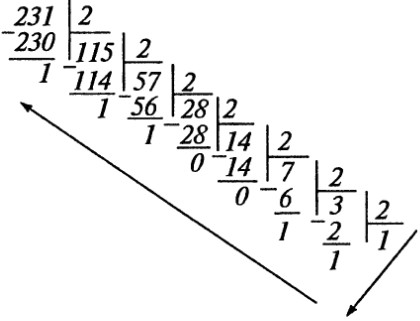
\includegraphics[height=10em]{image-001}

\textbf{Ответ}: $231_{(10)} = 11100111_{(2)}$
\end{frame}

\begin{frame}
\newgeometry{textwidth=30em}
\frametitle{Перевод из СС с основанием 2 в СС с основанием 4}
\textbf{Сложный путь}: 1) CC-2 -> CC-10: $10100_{(2)} = 20_{(10)}$\\
2) CC-10 -> CC-4: $20_{(10)} = 110_{(4)} => 10100_{(2)} = 110_{(4)}$\\
{\small Примечание: <<СС-N>> означает <<система счисления с основанием N>>}
\\ \hspace{\textwidth}
\bfseries{Простой путь}:\\
$x_{i+1}2^{i+1} + x_i2^i + \ldots + x_32^3 + x_22^2 + x_12^1 + x_02^0$\\
{\setstretch{1.4}
$x_{2k+1}2^{2k+1} + x_{2k}2^{2k} + \ldots + x_32^{2*1+1} + x_22^{2*1} + x_12^1 + x_02^0$\\
$2^{2k}(x_{2k+1}2^1 + x_{2k}) + \ldots + 2^2(x_32^1 + x_2) + 2^0(x_12^1 + x_0)$\\
$4^k(x_{2k+1}2^1 + x_{2k}) + \ldots + 4^1(x_32^1 + x_2) + 4^0(x_12^1 + x_0)$\\}
\vspace{3em}
\end{frame}

\begin{frame}
\frametitle{Преобразование из СС-2 в СС-2\textsuperscript{k} и обратно}
\begin{table}[]
\begin{tabular}{|c|c|c|}
\hline
\textbf{2-я <-> 4-я} & \textbf{2-я <-> 8-я} & \textbf{2-я <-> 16-я} \\ \hline
00 <-> 0 & 000 <-> 0 & 0000 <-> 0 \\ \hline
01 <-> 1 & 001 <-> 1 & 0001 <-> 1 \\ \hline
10 <-> 2 & 010 <-> 2 & 0010 <-> 2 \\ \hline
11 <-> 3 & 011 <-> 3 & 0011 <-> 3 \\ \hline
         & 100 <-> 4 & ... \\ \hline
         & 101 <-> 5 & 1101 <-> D \\ \hline
         & 110 <-> 6 & 1110 <-> E \\ \hline
         & 111 <-> 7 & 1111 <-> F \\ \hline
\end{tabular}
\end{table}

\textbf{Пример}: $1111110001,1110001_{(2)} = 0011 1111 0001,1110 0010_{(2)} = 3F1,E2_{(16)}$
\vspace{3em}
\end{frame}

\begin{frame}
\frametitle{Преобразование из CC-N в СС-N\textsuperscript{k} и обратно}
\textbf{Из СС-N в СС-N\textsuperscript{k}}
\begin{itemize}
    \setbeamertemplate{itemize items}[circle]
    \item дополнить число, записанное в СС с основанием $N$, незначащими нулями так, чтобы количество цифр было кратно $k$;
    \item разбить полученное число на группы по $k$ цифр, начиная от нуля;
    \item заменить каждую такую группу эквивалентным числом, записанным в СС с основанием $N^k$.
\end{itemize}
{\small
Задача: $1020101_{(3)} = ?_{(27)}$\\
Решение: $1020101_{(3)} = 001 020 101_{(3)} = 16A?_{(27)}$
}\\
\textbf{Из СС-N\textsuperscript{k} в СС-N}
\begin{itemize}
    \setbeamertemplate{itemize items}[circle]
    \item заменить каждую цифру числа, записанного в CC с основанием $N^k$, эквивалентным набором из $k$ цифр CC с основанием $N$.
\end{itemize}
{\small
Задача: $2345_{(125)} = ?_{(5)}$\\
Решение: $2345_{(125)} = 002 003 004 010_{(5)} = 2003004010_{(5)}$
}
\end{frame}
\end{document}
